\documentclass{article}
\usepackage[margin=0.8in]{geometry}
\usepackage{amsmath}
\usepackage{amssymb}
\usepackage{booktabs}
\usepackage{xintexpr}
\usepackage{tikz}
\usetikzlibrary{arrows,automata}
\usepackage{subcaption}
\usepackage{float}

\newcommand{\T}{1}
\newcommand{\F}{0}
\newcommand{\TF}[1]{\if1#1\T\else\F\fi}
\newcommand{\xintTF}[1]{\xintifboolexpr{#1}{\T}{\F}}

\newcommand{\logicrule}[2]{
\begin{array}{l}
#1 \\
\midrule
\therefore #2 \\
\end{array}
}

\newcommand{\inv}[1]{#1^{-1}}

\renewcommand{\d}[1]{\,\textnormal{d}#1}
\newcommand{\dd}[2]{\frac{\d{#1}}{\d{#2}}}
\newcommand{\ddd}[2]{\dfrac{\d{#1}}{\d{#2}}}

\DeclareMathOperator{\var}{Var}
\DeclareMathOperator{\E}{\mathcal{E}}

\newcommand{\multistep}[1]{\begin{array}{rl} #1 \end{array}}
\newcommand{\subeq}{\subseteq}
\newcommand{\sub}{\subset}

\newcommand{\conj}[1]{\overline{#1}}

\newcommand{\problem}[1]{$\boxed{\textbf{#1}}$}

\setlength\parindent{0pt}
\setlength\parskip{1em}

\begin{document}

\textbf{Tanner Hobson: thobson2}

\problem{1.1}

\begin{figure}[H]
\centering
\begin{subfigure}{.5\textwidth}
  \centering
  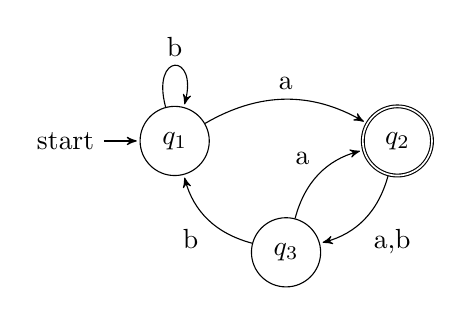
\begin{tikzpicture}[>=stealth',shorten >=1pt,auto,node distance=2cm]
    \node[initial,state] (q1)      {$q_1$};
    \node[state]         (q3) [below right of=q1] {$q_3$};
    \node[state,accepting]         (q2) [above right of=q3]  {$q_2$};

    \path[->]
    (q1) edge [loop above] node {b} (q1)
    (q1) edge [bend left] node {a} (q2)
    (q2) edge [bend left] node {a,b} (q3)
    (q3) edge [bend left] node {a} (q2)
    (q3) edge [bend left] node {b} (q1)
    ;
  \end{tikzpicture}
  \caption{$M_1$}
\end{subfigure}%
%
\begin{subfigure}{.5\textwidth}
  \centering
  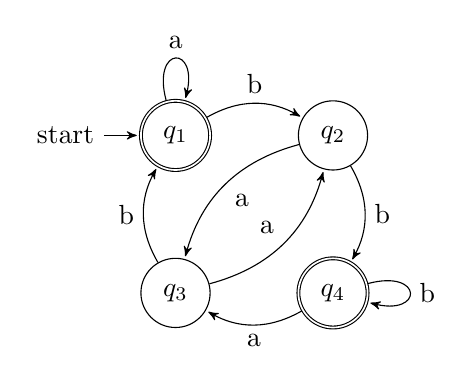
\begin{tikzpicture}[>=stealth',shorten >=1pt,auto,node distance=2cm]
    \node[initial,state,accepting] (q1)      {$q_1$};
    \node[state] (q2) [right of=q1] {$q_2$};
    \node[state]         (q3) [below of=q1] {$q_3$};
    \node[state,accepting]         (q4) [right of=q3]  {$q_4$};

    \path[->]
    (q1) edge [loop above] node {a} (q1)
    (q1) edge [bend left] node {b} (q2)
    (q2) edge [bend right] node {a} (q3)
    (q2) edge [bend left] node {b} (q4)
    (q3) edge [bend left] node {b} (q1)
    (q3) edge [bend right] node {a} (q2)
    (q4) edge [bend left] node {a} (q3)
    (q4) edge [loop right] node {b} (q4)
    ;
  \end{tikzpicture}
  \caption{$M_2$}
\end{subfigure}
\end{figure}

\begin{figure}[H]
  \centering
  \begin{tabular}{l|l|l}
    Part & $M_1$ & $M_2$ \\
    \hline
    a. & $q_1$ & $q_1$ \\
    b. & $\{q_2\}$ & $\{q_1,q_4\}$ \\
    c. &
    $q_1\rightarrow{}q_2\rightarrow{}q_3\rightarrow{}q_1\rightarrow{}q_1$ &
    $q_1\rightarrow{}q_1\rightarrow{}q_1\rightarrow{}q_2\rightarrow{}q_4$ \\
    d. & No & Yes \\
    e. & No & Yes \\
  \end{tabular}
\end{figure}

\problem{1.2}

The machines can be formally represented as:

\[
\begin{array}{l|l|l}
& M_1 & M_2 \\
\midrule
Q & \{q_1,q_2,q_3\} & \{q_1,q_2,q_3,q_4\} \\
\Sigma & \{a,b\} & \{a,b\} \\
\delta & \delta_1 & \delta_2 \\
q_0 & q_1 & q_1 \\
F & \{q_2\} & \{q_1,q_4\} \\
\end{array}
\]

where the $\delta$ functions are

\begin{figure}[H]
\centering
\begin{subfigure}{.5\textwidth}
  \centering
  $
  \begin{array}{l|l|l}
    q_i & q_{i+1}\text{ if a} & q_{i+1}\text{ if b} \\
    \midrule
    q_1 & q_2 & q_1 \\
    q_2 & q_3 & q_3 \\
    q_3 & q_2 & q_1 \\
  \end{array}
  $
  \caption{$\delta_1$}
\end{subfigure}%
%
\begin{subfigure}{.5\textwidth}
  \centering
  $
  \begin{array}{l|l|l}
    q_i & q_{i+1}\text{ if a} & q_{i+1}\text{ if b} \\
    \midrule
    q_1 & q_1 & q_2 \\
    q_2 & q_3 & q_4 \\
    q_3 & q_2 & q_1 \\
    q_4 & q_3 & q_4 \\
  \end{array}
  $
  \caption{$\delta_2$}
\end{subfigure}
\end{figure}

\problem{1.3}

\begin{figure}[H]
  \centering
  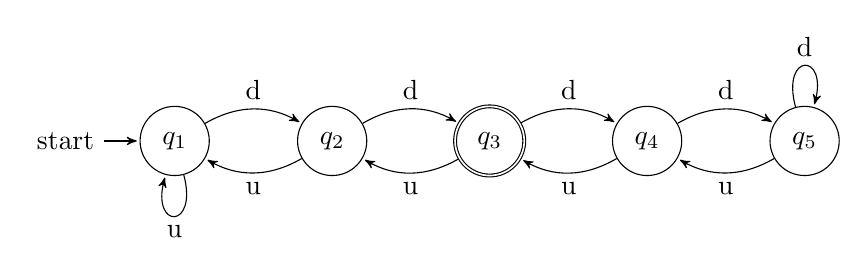
\begin{tikzpicture}[>=stealth',shorten >=1pt,auto,node distance=2cm]
    \node[initial,state] (q1)      {$q_1$};
    \node[state] (q2) [right of=q1] {$q_2$};
    \node[state,accepting]         (q3) [right of=q2] {$q_3$};
    \node[state]         (q4) [right of=q3]  {$q_4$};
    \node[state]         (q5) [right of=q4]  {$q_5$};

    \path[->]
    (q1) edge [loop below] node {u} (q1)
    (q1) edge [bend left] node {d} (q2)

    (q2) edge [bend left] node {u} (q1)
    (q2) edge [bend left] node {d} (q3)

    (q3) edge [bend left] node {u} (q2)
    (q3) edge [bend left] node {d} (q4)

    (q4) edge [bend left] node {u} (q3)
    (q4) edge [bend left] node {d} (q5)

    (q5) edge [bend left] node {u} (q4)
    (q5) edge [loop above] node {d} (q5)
    ;
  \end{tikzpicture}
\end{figure}

\end{document}
